%this is the DQC1 presentation

\documentclass{article}
\usepackage{etex}
\usepackage{amsmath}
\usepackage{braket}
\usepackage{tikz}
\usepackage{braids}
\usepackage{qcircuit}
\begin{document}
\title{DQC1 complexity class and Jones polynomials} 
\author{Ohad Barta}
\date{\today} 

\titlepage
\tableofcontents



\section{DQC1 class and DQC1-complete problems}
\subsection{DQC1 class definition  } 
\title{DQC1 class definition} 
DQC1 class is the class of decidable languages with algorithm $A$ such that:
\begin{itemize}
\item $A$ starts with one clean qubit in state $\ket{0}$, and $n$ qubits in the maximally mixed state
\item $A$ may perform any unitary operation
\item $A$ can only perform a measurement of the clean qubit at the end of the algorithm
\item $A$ has no access to a classical computer, so its not promised that $P \subset DQC1$ 
\item $A$ cannot be invoked many times in parallel
\item $A$ runs in polynomial time
\item $\forall x$, $A$ decides if $x \in L$ correctly with probability of at least $\frac{2}{3}$
\end{itemize}


\title{Complete Problems definition} 
Reminder: in general, a language L is said to be "complete" in the class DQC1, if:
\begin{itemize}
\item $L \in DQC1$
\item $\forall L_{0} \in DQC1$ there is a reduction from $L_{0}$ to L, such that the reduction algorithm is in DQC1  
\end{itemize}
In the next few slides, we show that calculating an estimate of the trace of a unitary matrix is DQC1-complete


\subsection{trace estimation algorithm  }
\title{trace estimation algorithm (1)}
The start state of any DQC1 problem is one clean qubit (state $\ket{0}$), and n-qubits in the maximally mixed state.
That is, the start state is
\begin{equation}
\rho = \ket{0}\bra{0}\otimes\frac{I}{2^n}
\end{equation}
We can use the Hadamard test, which gets as input this state, in order to accurately estimate a trace
of a unitary operation U.


\title{The Hadamard Test}
The description of the Hadamard test for some unitary matrix U is:
\\\\
\Qcircuit @C=1em @R=.7em {
	\lstick{\ket{0}} & \gate {H} & \ctrl{1} & \gate {H} & \meter & \qw \\
	\lstick{\psi} & {/} \qw & \gate {U} & {/} \qw & \qw & \qw
}
\\\\\\
We will show that this circuit indeed calculates the trace of U
\begin{itemize}
\item after the first Hadamard gate, the state is $\Ket{+}\psi = \frac{1}{\sqrt{2}}\Ket{0}\Ket{\psi} + \frac{1}{\sqrt{2}}\Ket{1}\Ket{\psi}$
\item after the C-U operation, the new state is $\frac{1}{\sqrt{2}}\Ket{0}\Ket{\psi} + \frac{1}{\sqrt{2}}\Ket{1}U\Ket{\psi}$
\item after the final Hadamard operation, the final state becomes $\frac{1}{2}\Ket{0}\Ket{\psi} + \frac{1}{2}\Ket{1}\Ket{\psi}\ +\frac{1}{2}\Ket{0}U\Ket{\psi}\ -  \frac{1}{2}\Ket{1}U\Ket{\psi} = 
\frac{\Ket{\psi} + U\Ket{\psi}}{2}\Ket{0} + \frac{\Ket{\psi} - U\Ket{\psi}}{2}\Ket{1}$
\end{itemize}

 \title {The Hadamard Test (2) }
 Therefore, the probability for measuring 0 at the end of the calculation is:
 $ \rho_{0} = (\frac{\Bra{\psi} + \Bra{\psi}{U^\dagger}}{2})(\frac{\Ket{\psi} + U\Ket{\psi}}{2}) = 
  \frac{1}{4}(\Bra{\psi}\Ket{\psi} + \Bra{\psi}{U^\dagger}\Ket{\psi} + \Bra{\psi}U\Ket{\psi} + \Bra{\psi}{U^\dagger}U\Ket{\psi}  )
  = \frac{1}{2} + \frac{1}{4}(\Bra{\psi}{U^\dagger}\Ket{\psi} + \Bra{\psi}U\Ket{\psi})
  =  \frac{1}{2} +  \frac{1}{2}Re(\Bra{\psi}U\Ket{\psi}) $
  When we remember that in our case $\psi$ is actually the completely mixed state, we get that the probability is:
  \begin{displaymath}
  \frac{1}{2^{n}}\sum\limits_{\psi \in {0,1}^n} \frac{1+Re(\Bra{\psi}U\Ket{\psi})}{2} = \frac{1}{2} + \frac{Re(TrU)}{2^{n+1}}
\end{displaymath}
Therefore, the problem of trace estimation can be solved with one clean qubit.

\subsection{Hardness of trace estimation}
\title {The hardness of trace estimation}
Next, we will want to show that trace estimation is hard in DQC1.
Suppose we have some language $L \in DQC1$, and some x, and we want to decide if $x \in L$.

$L \in DQC1$, therefore its start state obeys equation 1. on this start state, we apply some unitary matrix U, and get the state $\rho_{final} = U\rho{U^\dagger} = U\ket{0}\bra{0}\frac{I}{2^n}{U^\dagger}$
Therefore, the probability to measure 0 is equal to the trace of the submatrix of the final matrix in which the first qubit is in state $\ket{0}$:
\begin{equation}
 p_{0} = Tr[\Ket{0}\Bra{0}\otimes I\rho_{final}] = 2^{-n}Tr[(\Ket{0}\Bra{0}\otimes I)U(\Ket{0}\Bra{0}\otimes I{U^\dagger})]
\end{equation}
Unfortunately - this matrix isn't unitary!!

%% proof - $AU(AU)^\dagger=AUU^\daggerA^\dagger=AA^\dagger \ne I

\title{The hardness of trace estimation (2)}
To resolve this issue, we examine the following quantom circuit C:
\\
\Qcircuit @C=1em @R=.7em {
	& \qw & \multigate{1}{U^\dag} & \ctrl{2} & \multigate{1}{U} & \ctrl{3} & \qw \\
	& {/} \qw & \ghost{U^\dag} & \qw & \ghost{U} & \qw &  {/} \qw \\
	&  \qw &\qw &  \targ  & \qw & \qw \\
	&  \qw & \qw & \qw & \qw & \targ & \qw
}
\\
Proposition 1.1: $\frac{1}{4}$tr[C]=$Tr[(\Ket{0}\Bra{0}\otimes I)U(\Ket{0}\Bra{0}\otimes I{U^\dagger})]$

Proof:
\begin{itemize}
\item first, lets remember that $tr[C] = \sum\limits_{\psi \in {0,1}^n} \Bra{\psi}C\Ket{\psi}$
and in a similar way, $Tr[(\Ket{0}\Bra{0}\otimes I)U(\Ket{0}\Bra{0}\otimes I{U^\dagger})] = \sum\limits_{\psi \in {0,1}^n} \Bra{\psi}(\Ket{0}\Bra{0}\otimes I)U(\Ket{0}\Bra{0}\otimes I{U^\dagger})\Ket{\psi}$
\end{itemize}

\title{The hardness of trace estimation (3)}
\begin{itemize}
\item that is, some state $\psi$ contribute to the trace of D iff after imply $U^\dagger$ it has some
component with zero in its first qubit, and then after implying U on that component, we still remain with some non-zero component in the first qubit
\item Similarly, in C, if, say, the result of implying $U^\dagger$ on $\psi$ give a non-zero component, the one of the two last qubits will "flip", creating a state orthogonal to the original state
(and similarly on U).
\item therefore, the two circuits traces has the exact same components and are equal, up to factor of 4
(which come from the "free choice" in the values of the two last qubits in C)
 
\end{itemize}

\subsection{adding few more clean bits don't give extra power}
\title{adding few more clean bits don't give extra power}
We showed that computing the matrix trace is DQC1-complete problem.
We notice now that actually we didn't computed it accurately. Since only the expectation off the algorithm is the trace, we rather get an approximation. According to the Chernoff inequality, the approximation will be exponentially  good with polynomial number of repetitions. However here the matrix is exponentially large, so we get an approximation of $\frac{1}{poly(n)}$ to the expression $\frac{Tr(U)}{2^{n+1}}$, or  in other words we have a $\frac{2^{n}}{poly(n)}$ additive- approximation to the trace. 


\title{adding few more clean bits don't give extra power (2)}
We will define now the DQCK complexity class:
DQCK class is the class of decidable languages with algorithm A such that:
\begin{itemize}
\item A runs in polynomial time
\item $\forall x$, A decide correctly if $x \in L$, with probability of at least $\frac{2}{3}$. 
In case that $x \in L$, we expect the first clean qubit to be 0 at the end of the algorithm
\item A start state includes K clean qubits (K can be a constant, or a function of n) (state $\ket{0}$), and n-qubits in the maximally mixed state
\item A may perform any unitary operation on his start state
\item A can measure only the clean qubits, only at the end of the algorithm
\item We assume that A is invoked cant be invoked many times in parallel
\item A has no access to classical computer, so its not promised that $P \subset DQCK$ 
\end{itemize}  


\title{adding few more clean bits don't give extra power (3)}
We will now prove that for $k \leq \log{n}$, estimate the trace of unitary matrix with the same precision is still a complete problem, thus proving that adding logarithmic number of clean bits doesn't change the power. 

Obviously we can calculate the trace of unitary matrix with $\log{n}$ bits, since we can do it just with one. 


\title{adding few more clean bits don't give extra power (3)}
As for the less trivial direction, assume we have some quantum algorithm in DQCK.
Similarly to the one-qubit option, final state is:
$\rho_{final} = U\rho{U^\dagger} = U{\ket{0}\bra{0}}^{\otimes k}\frac{I}{2^n}{U^\dagger}$
and therefore the probability of measuring 0 at the end is:
$p_{0} = Tr[{\Ket{0}\Bra{0}}^{\otimes k} \otimes I\rho_{final}] = 2^{-n}Tr[(\Ket{0}\Bra{0}\otimes I)U({\Ket{0}\Bra{0}}^{\otimes k}\otimes I{U^\dagger})$

Now, we have the same problem at estimating this matrix: its not unitary!
To resolve that issue, we build circuit similar to the one in the 1-clean qubit process,
but now we add 2k ancilla qubits, when there is a CNOT gate between each i-th qubit and (i+k)-th qubit.



\title{adding few more clean bits don't give extra power (4)}
Now, we can see (similarly to the proposition 1.1), that the trace of the new circuit $U^{*}$ follows the rule: $Tr[U^{*}] = 2^{k}Tr[U]$. Thus, in polynomial number of executions we can compute its trace up to a precision of $\frac{2^{n+k}}{poly(n,k}$, but this equals to $\frac{2^{n}}{poly(n}$ when $k  \leq \log{n}$, which means that in this case the precision is good enough to decide the original problem.



\section{DQC1 algorithm for evaluating Jones Polynomial}
\subsection{Knots, Braid groups and Temperley-Lieb Algebra}
\subsubsection{Knots}
\title{Knots}
A knot is one strand, in $R^3$. The knot is invariant to moving or stretching, but we cant cut the knot.
An old topology question, is to know if two knots are actually the same knot.Reidemeister showed in 1927
the "Reidemeister moves", which doesn't change the knot.
\begin{figure}
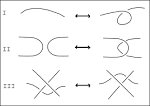
\includegraphics[scale=0.5]{Reidemeister} 
\caption{Reidemeister moves}
\end{figure}

  
\subsubsection{Braid groups}
\title{Braid groups}
\begin{definition}
Consider two horizontal bars, one on top of the other, with n-points each. A n-stand braid, is
n strands, such that:
\begin{itemize}
\item each strand has exactly one peg attached to it on each bar
\item the strands may cross one over another
\item at every point, the strand direction has non-zero component directed down 
\end{itemize}
\end{definition}

We call to the collection of all such braids the braid group $B_{n}$, with identity element and generators that will immediately follow, when the operation between two brands is put them one below the other, and connect all the button-pegs of the first, with the top-pegs of the second.

\title{examples}
The identity braid:
\begin{center}
\begin{tikzpicture}
\braid[rotate=0,number of strands = 3, style strands={1}{ red } ,style
strands={2}{ blue } ,style strands={3}{ green } ]; 
\end{tikzpicture}
\end{center}

Some other braid:
\begin{center}
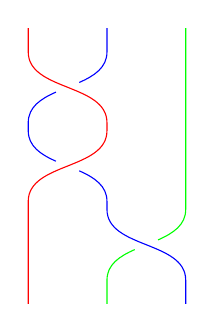
\begin{tikzpicture}
\braid[rotate=0, style strands={1}{ red } ,style
strands={2}{ blue } ,style strands={3}{ green } ] s_1 s_1^{-1} 
s_2;
\end{tikzpicture}
\end{center}
 


\title{braid group generators}
$\forall 1\leq i \leq n$, we denote by $\sigma_{i}$, the braid which takes the i-th strand
to the (i+1) place, the (i+1)-strand to the i-th place, and leaves all the other strands in place.
For example, this is $\sigma_{2}$ with 3-strands:
\begin{center}
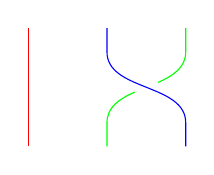
\begin{tikzpicture}
\braid[rotate=0, style strands={1}{ red } ,style
strands={2}{ blue } ,style strands={3}{ green } ]s_2;
\end{tikzpicture}
\end{center}

Notice that when $1 < |i - j|$ then $\sigma_{i}, \sigma_{j}$ act on completely different strands, so they are commutative: $\sigma_{i}\sigma_{j} = \sigma_{j}\sigma_{i}$

Furthermore, it holds that $\sigma_{i}\sigma_{i+1}\sigma_{i} = \sigma_{i+1}\sigma_{i}\sigma_{i+1}$
(both switch the i-th strand and the (i+2)-strand, while leave all the others in place)


\title{braid groups and knots}
Braids can create a knot by "joining the loose ends" all together. there are two ways of doing it:
The plat closure, where we join neighbour pegs in the top and bottom, and the trace closure, where we connect each top peg to the corresponding bottom peg, without creating more loops.
for example, for the following braid: 

\begin{center}
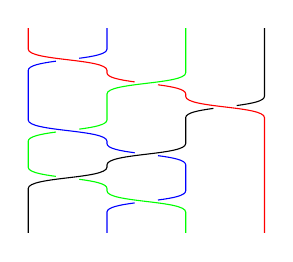
\begin{tikzpicture}
\braid[rotate=0, height=.3cm, style strands={1}{ red } ,style
strands={2}{ blue } ,style strands={3}{ green } ,style strands={4}{ black } ] s_1 s_2^{-1} 
s_3 s_1 s_2^{-1} s_1^{-1} s_2;
\end{tikzpicture}
\end{center} 
has this closures:
\begin{figure}
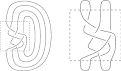
\includegraphics[scale=0.5]{closures} 
\caption{plat and trace closures}
\end{figure}



\subsubsection{Temperley-Lieb-algebra}
\title{Temperley-Lieb algebra}
In a similar way to the braid groups, we can define the Temperley-Lieb {n,d} algebra.
Temperley-Lieb {n,d} algebra group consists of two rows of pegs (button and top), and n-strands, such that:
\begin{itemize}
\item each strand connects to exactly two pegs (but they can be from the same side!)
\item the strands cannot intersect between them.
\item the operator of two objects like this is simply put them one below the other, 
while erasing circuits created, but multiply the final result by d, for each circuit removed
\end{itemize}
an example for this operator is:
\begin{figure}
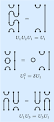
\includegraphics[scale=0.5]{tempely_lieb_operator} 
\caption{plat and trace closures}
\end{figure}


\title{Temperley-Lieb algebra generators}
In a similar way to the braid groups, we can define generators to the this algebra, 
such that the $i$th generator send the $i$th strand on the bottom and top the the i+1 peg, 
and leaves all the others in place.
\begin{figure}
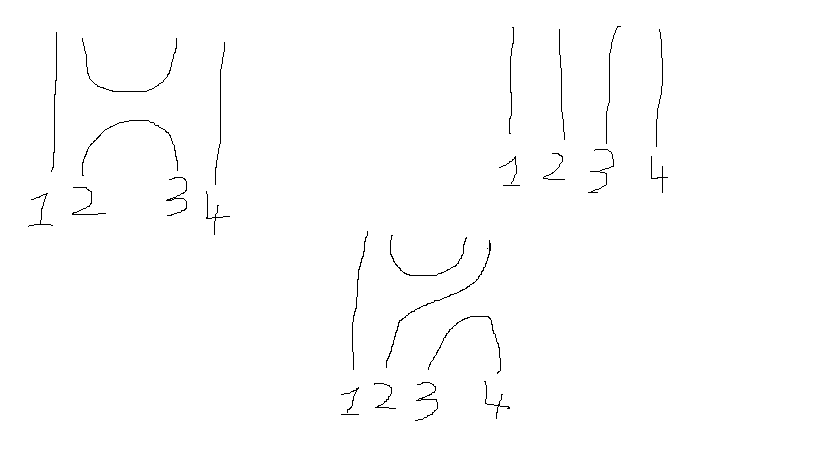
\includegraphics[scale=0.5]{tempely_lieb_generators} 
\caption{Temperley-Lieb generators}


\end{figure}
Notice that these generators obeys the following rules (as demonstrated in the previous slide figure):
\begin{itemize}
\item $E_{i}E_{j} = E_{j}E_{i}$, when $2 \leq |i-j$
\item $E_{i}E_{i+1}E_{i} = E_{i}$, $E_{i}E_{i-1}E_{i} = E_{i}$
\item ${E_{i}}^2 = dE_{i}$
\end{itemize}


\subsubsection{From braid groups to Temperley-Lieb algebra }
\title{From braid groups to Temperley-Lieb algebra}
Now, we observe that a connection between the braid groups and the Temperley-Lieb algebra can
be made by defining homomorphism to the braid groups generators. we will define:
$\rho_{A}(\sigma_{i}) = AE_{i} +A^{-1}I$, when I is the identity in the Temperley-Lieb algebra,
and A is a number that satisfies $A^{2}+A^{-2}=d$.
We can show that this is indeed a representation of the braid groups, if we show that the relations
of the braid group generators still hold.
As for the first relation, it holds that for $2 \leq |i-j|$ , $\rho_{A}(\sigma_{i}),\rho_{A}(\sigma_{j})$ commutes since in this case $E_{i},E_{j}$ commutes as well.

\title{From braid groups to Temperley-Lieb algebra (2)}
For the second relation, to show that :
\begin{displaymath}
\rho_{A}(\sigma_{i})\rho_{A}(\sigma_{i+1})\rho_{A}(\sigma_{i})= \rho_{A}(\sigma_{i+1})\rho_{A}(\sigma_{i})\rho_{A}(\sigma_{i+1})
\end{displaymath}
or:

$
A^{3}E_{i}E_{i+1}E_{i} +AE_{i}E_{i+1} + AE_{i}^{2} + A^{-1}E_{i} +AE_{i+1}E_{i}+A^{-1}E_{i+1} + A^{-1}E_{i} + A^{-3}$

=

$
A^{3}E_{i+1}E_{i}E_{i+1} +AE_{i+1}E_{i} + AE_{i+1}^{2} + A^{-1}E_{i+1} +AE_{i}E_{i+1}+A^{-1}E_{i} + A^{-1}E_{i+1} + A^{-3}
$
after delete similar elements and use some generators identities, we have to show that:
\begin{displaymath}
(A^{-1}+Ad+A^{3})E_{i}= (A^{-1}+Ad+A^{3})E_{i+1}
\end{displaymath}
and this is correct since $(A^{-1}+Ad+A^{3}) = 0$



\subsubsection{The Markov Trace}
\title{The Markov Trace}
The Markov Trace is a function on a Temperley-Lieb algebra, which defined as follows:
\begin{itemize}
\item given a Temperley-Lieb algebra object, we connect its bottom and top bars, in a similar way to
a trace closure.
\item when denote the number of loops created like this with a, the trace closure is $d^{a-n}$
\end{itemize}
The Markov trace Tr obeys the following:
\begin{itemize}
\item Tr[1] = 1 (the identity Temperley-Lieb algebra has n loops in its closure, $d^{n-n} = 1$)
\item $\forall X,Y \in TL[n,d]$, Tr[XY] = Tr[YX] 
\item $\forall X \in TL[n-1, d], Tr[xE_{n-1}]=\frac{Tr[x]}{d}$ (add $E_{n-1}$ add new peg but don't enlarge the number of loops).
\end{itemize}


\title{The uniqueness of the Markov Trace}
We will prove that the Markov trace is the only function on Temperley-Lieb objects that obeys rules 1-3,
By prove that rules 1-3 are enough to determine the trace value of any Temperley-Lieb object.
We will regard each object as a word with letter from the the group $E_{1}...E_{n}$
We will define such word to be "reduced", if it wont be equal to any "shorter" word.
The proof is done in induction on n, the maximal generator index in the reducible word:
\begin{itemize}
\item As for the base case, there is only one object with maximal generator 0 - the identity object, and its value is set to 1.
\item assume that the value is well defined for any reducible object maximal generator $\leq n$ and lets prove it for n+1. 
\end{itemize}


\title{The uniqueness of the Markov Trace (2)}
First, we will prove that in any such reducible word contains exactly one $E_{n}$ generator.
This will suffice, since then we can write $w=w_{1}E_{n}w_{2}$, when $w_{1}, w_{2}$ are
reducible words with maximal generator n-1, which their value is well defined by the induction assumption.

Then, it holds that $Tr[w]=Tr[w_{1}E_{n}w_{2}] = Tr[w_{1}w_{2}E_{n}] = dTr[w_{1}w_{2}]$, and
since $w_{1}w_{2}$ is another reducible word that its value is well defined, the proof will be complete.   


\title{The uniqueness of the Markov Trace (3)}
Assume the contrary, that is there is a reducible word that contains two $E_{n}$.
Then, we can write $w=w_{1}E_{n}w_{2}E_{n}w_{3}$, when $w_{i}$ are reducible with maximal generator
$E_{n-1}$. Now, if $E_{n-1}$ isn't in $w_{2}$, we can change the order (from generators rules:)
$w=w_{1}w_{2}E_{n}E_{n}w_{3}\ = dw_{1}w_{2}E_{n}w_{3}$,so w isn't reducible.
If there is $E_{n-1}$ in  $w_{2}$, we can write:
\begin{displaymath}
 w=w_{1}E_{n}v_{1}E_{n-1}v_{2}E_{n}w_{3},
 \end{displaymath} 
 when 
 $v_{i}$  are reducible with maximal generator
$(E_{n-2}$. Therefore, they can commute with $E_{n-1}$, creating 
\begin{displaymath}
w=w_{1}v_{1}E_{n}E_{n-1}E_{n}v_{2}w_{3}
= w_{1}v_{1}E_{n}v_{2}w_{3}
 \end{displaymath} 
 , so w again is not reducible
   



\subsection{Jones Polynomials} 
\subsubsection{The Kauffman Bracket Polynomial}
\title{Introduction}
After half a century of searching knots invariants in a geometric way, in 1984 the Jones polynomial
was discovered. It matches each knot a polynom , that stays invariant under the Reidemeister moves.
We will first define the Kauffman Bracket Polynomial, which is "almost" correct.

Consider a knot K. for each crossing in K, from the form 
\begin{center}
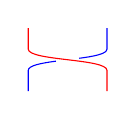
\begin{tikzpicture}
\braid[rotate=0, height=.3cm, style strands={1}{ red } ,style
strands={2}{ blue } ] s_1;
\end{tikzpicture}
\end{center} 

We decide at random to replace it with $E_{1}$, or with the Temperley-Lieb identity element.
Each decision like this for all the crossings is a state $\sigma$

\title{The Kauffman Bracket Polynomial - definition} 
We denote by $\sigma_{+}$ the number of replaces we made with $E_{1}$, and by 
$\sigma_{-}$ the number of replaces we made with the identity element.
We denote by$N_{\sigma}$ the number of loops created when all the changes of $\sigma$ are applied.
Then, the Kauffman Bracket Polynomial is defined as:
$ L(A) = \sum\limits_{all_states_\sigma}{A^{\sigma_{+}} A^{-\sigma_{-}}d^{N_{\sigma} - 1}}$

d is defined as: $d = -A^{-2} -A^2$ 



\title{The Kauffman Bracket Polynomial - properties} 
Note that the  Kauffman Bracket Polynomial holds the following rules:
\begin{itemize}
\item $\forall A$, L(A)=1 in the unknot (one state with $\sigma_{+}=0,\sigma_{-}=0, N_{\sigma} = 1$)
\item 
\begin{figure}
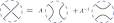
\includegraphics[scale=1]{Kauffman_bracket_identity} 
\caption{Kauffman bracket recursive nature}
\end{figure}
This comes directly from the definition, if we consider only one cross, after choose a state sigma for all the others, or we choose to replace it with $E_{1}$ and multiply by A, or we choose to replace it by the identity and multiply by $A^{-1}$
\item we can eliminate an isolated unknot and multiply the result with a factor of d. (examples will follow). 
\end{itemize}


\subsubsection{The Jones Polynomial}
\title{definition}
Jones polynomial is different from Kauffman bracket polynomial only with some normalization factor.
We define by the w(k) for a knot k to be: $w(k) = \sum\limits_{all crossings}{(-1)^{is the left arrow above the right one}}$
and Jones polynomial is defines as: $V_{k}(t)=V_{k}(A^{-4})=(-A)^{3w(k)}L_{k}(A)$.

Notice that w(k) for the unknot is 0, so the Jones polynomial of the unknot is still equals to 1 at any point.



\title{example}
Lets see an example to the calculation of Kauffman and Jones polynomial. Consider the Hopf link.
The Kauffman polynomial of this link is:
\begin{figure}
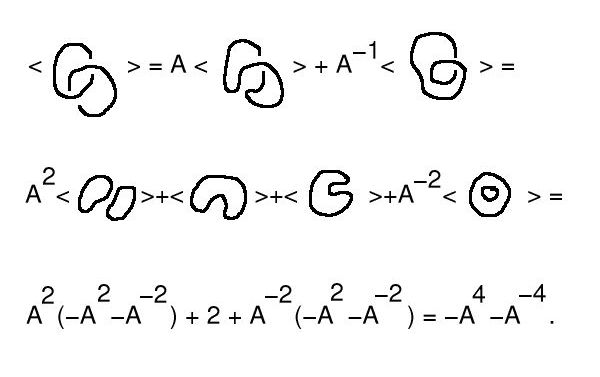
\includegraphics[scale=0.15]{hopf_link} 
\caption{the Kauffman polynomial of the Hopf link}
\end{figure}

Moving to Jones Polynomial, we can see that w(Hopf Link)=-2 (two cross with the same orientation), so:
$V_{hopfLink}=(-A)^{-6}(A^{-4}+A^{4}) = A^{-2} + A^{-10})$.
Remember that $t = A^{-4}$ and we get $V_{hopfLink}(t)=\sqrt{t}(1+t^{2})$  



\title{the connection to Reidemeister moves}
For Completion, we will note that it is easy to see that Jones Polynomial remains the same
under Reidemeister moves. We will show here only one of the three, the others can be proved in a similar technique:
\begin{figure}
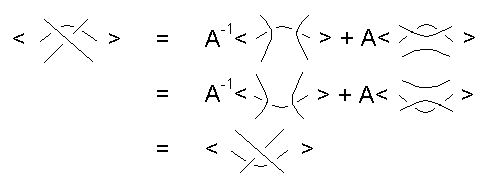
\includegraphics[scale=1]{jones_and_reidimister.jpg} 
\caption{the Kauffman polynomial of the Hopf link}
\end{figure}  


\title{the connection to Markov trace and braid groups}
We will now show a connection between the Jones Polynomial and the Markov trace.
Proposition:
$V_{B^{tr}}(A) = (-A)^{3w(B^{tr})}d^{n-1}Tr[\rho_{A}(B)]$
That is, the Jones polynomial of a trace-closure of some braid is connected to the Markov trace value of its corresponding Temperley-Lieb object.
Proof:

We only have to proof that $L(B^{tr}) = d^{n-1}Tr[\rho_{A}(B)]$. Recall that for each crossing in the braid B, the Kauffman polynomial hold \begin{figure}
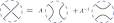
\includegraphics[scale=1]{Kauffman_bracket_identity} 
\caption{Kauffman bracket recursive nature}
\end{figure}.
The homomorphism also has the form of  $\rho_{A}(\sigma_{i}) = AE_{i} +A^{-1}I$ - exactly the same!.

\title{the connection to Markov trace and braid groups(2) }
After choosing a state $\sigma$, its value in the Kauffman polynomial is $d^{N_{\sigma} -1)}$, and its
value i the Markov trace is $d^{N_{\sigma}} -n )$, therefore we need the $d^{n-1}$ factor. 
 

\subsection{The Fibonacci representation}
\title{The Fibonacci representation of a braid group}
We would like to obtain some matrix representation of a braid. Given an n-strand braid, we can write a string of n+1 elements on the bottom of the braid between every two strands, where each element is either * or p. The only restriction is that there will be no two adjacent * elements. The number of possibilities to do so is of course $f_{n+3}$, where $f_{n}$ denotes the $n$th Fibonacci number.

Next, for each crossing and labelling of it (the 3 elements from the right, left, and in the crossing) , we would like to give a linear function that will "open up" the crossing, and that may change the center label. (we wouldn't want to change the right or left label, in order to preserve the string of elements correctness under all the operations).
 

\title{The Fibonacci representation of a braid group (2)}
That is, in the most general form, a cross $\sigma_{i}$ with labeling of P*P, can move to 
a times * Identity with labelling P*P + b times the identity with labelling PPP.
we will denote it by $(p\hat{*}p)=a(p*p)+b(ppp)$


Such matrix representation must have some properties that will make it useful to us:
\begin{itemize}
\item for every braid, its matrix must be unitary, so we can link it to some quantom circuit.
\item for every braid, there has to be some connection between the Jones Polynomial of the braid, and the relevant matrix.
\end{itemize}
 


\title{The Fibonacci representation of a braid group (3)}
The explicit representation is:
$(*\hat{p}p)=a(*pp)$

$(*\hat{p}*)=b(*p*)$

$(p\hat{*}p)=c(p*p)+d(ppp)$

$(p\hat{p}*)=a(pp*)$

$(p\hat{p}p)=d(p*p)+e(ppp)$

, with:
$ a = -A^{4} $


 $  b = A^{8}  $
 
 $  c = A^{8}\tau^{2} - A^{4}\tau $
  
 $  d = A^{8}\tau^{\frac{3}{2}} + A^{4}\tau^{\frac{3}{2}} $ 
 
 $  e = A^{8}\tau - A^{4}\tau^{2} $ 
 
 $  A = e^{\frac{-3{\pi}i}{5}} $ 
 
 $  \tau = \frac{2}{1 + \sqrt{5}} $


 
\title{The Fibonacci representation - example}
We will show the Fibonacci representation of $\sigma_{1}$ with 3 strands:
\[
\begin{pmatrix} b & 0 & 0 & 0 & 0 & 0 & 0 & 0 \\ 0 & a & 0 & 0 & 0 & 0 & 0 & 0 \\ 0 & 0 & a & 0 & 0 & 0 & 0 & 0 \\ 0 & 0 & 0 & e & 0 & d & 0 & 0 \\ 0 & 0 & 0 & 0 & a & 0 & 0 & 0 \\ 0 & 0 & 0 & d & 0 & e & 0 & 0 \\0 & 0 & 0 & 0 & 0 & 0 & e & d \\0 & 0 & 0 & 0 & 0 & 0 & d & c \end{pmatrix} 
  \begin{pmatrix} *p*p \\ *ppp \\ *pp* \\ pppp \\ pp*p \\ pp*p \\ p*pp \\ ppp* \\ p*p* \end{pmatrix}
\]

\subsubsection{Unitarity}
\title{The Unitary of the Fibonacci representation}
Its enough to prove that all the braid group generators, since multiplication of unitary matrices is again unitary matrix. Each generator like this include only one cross. As we saw in the definition and examples, each cross leaves only 1-2 non-zero elements in each matrix row, in the corresponding labelling entry.

we will move onto the 5 options to label the 3 elements near the cross (since the other elements doesn't matter here).
\begin{itemize}
\item with all the labelling with the form ...*pp... , the unitary row will include only one "a" in the matrix diagonal, and no other row have non-zero entries in that column. That is, with multiplied by its dagger, the entry on the diagonal will be $a^{\dagger}a = e^{\frac{-12{pi}i}{5}}e^{\frac{12{pi}i}{5}} = 1$, and all the other entries will be zero.
\item the same reasoning apply for labeling with the form ...pp*...  
\end{itemize}


\title{The Unitary of the Fibonacci representation (2) }
\begin{itemize}
\item with all the labelling with the form ...*p*... , the unitary row will include only one "b" in the matrix diagonal, and no other row have non-zero entries in that column. That is, with multiplied by its dagger, the entry on the diagonal will be $b^{\dagger}b = e^{\frac{-24{pi}i}{5}}e^{\frac{24{pi}i}{5}} = 1$, and all the other entries will be zero.
\item  with all the labelling with the form ...p*p.., the unitary row will include one "d" in the ...ppp.. entry, and one "c" in the ...p*p.. entry. that is, when multiplied by its dagger, the diagonal element will be $c^{\dagger}c + d^{\dagger}d = (A^{-8}\tau^{2} - A^{-4}\tau)(A^{8}\tau^{2} - A^{4}\tau) + (A^{-8}\tau^{\frac{3}{2}} + A^{-4}\tau^{\frac{3}{2}})(A^{8}\tau^{\frac{3}{2}} + A^{4}\tau^{\frac{3}{2}})$

$ = \tau^{4} - A^{-4}\tau^{3} - A^{4}\tau^{3} + \tau^{2} + \tau^{3} + A^{-4}\tau^{3} + A^{4}\tau^{3} + \tau^{3}$

$ = \tau^{4} + 2\tau^{3} + \tau^{2} = {\tau^{2}(\tau+1)}^{2} = 1^{2} = 1$ 
\end{itemize}


\title{The Unitary of the Fibonacci representation (3) }
\begin{itemize}
\item  now, lets check another entries in this row, after multiply this matrix by its dagger.
All the other rows has zero entries in the relevant columns, except the ...ppp.. row. when multiply, we will get $e^{\dagger}d + d^{\dagger}c = (A^{-8}\tau - A^{-4}\tau^{2})(A^{8}\tau^{\frac{3}{2}} + A^{4}\tau^{\frac{3}{2}}) + (A^{-8}\tau^{\frac{3}{2}} + A^{-4}\tau^{\frac{3}{2}})(A^{8}\tau^{2} - A^{4}\tau)$

$ = \tau^{2.5} + A^{-4}\tau^{2.5} - A^{4}\tau^{3.5} - \tau^{3.5} + \tau^{3.5} - A^{-4}\tau^{2.5} + A^{4}\tau^{3.5} - \tau^{2.5}$

$ = 0$
\item similar calculation will yield the result on the ...ppp... rows   
\end{itemize}

\subsubsection{Fibonacci representation and Jones Polynomial}
\title{Fibonacci representation and Jones polynomial}
We will want to connect somehow between the Fibonacci representation and the Jones Polynomial.
For this, we will use the Temperley-Lieb algebra, and the Markov Trace. We saw that the Markov trace
is a uniquely defined function over the Temperley-Lieb algebra, such that it is strongly connected to the Jones Polynomial. If we will be able to define a function over the Fibonacci representation that "behaves the same", we will be able to show such correlation between Jones Polynomial and the Fibonacci representation. We will donate this function as $\tilde{Tr}$


\title{Fibonacci representation and Jones polynomial (2)}
The requirements from  $\tilde{Tr}$ are:
\begin{itemize}
\item $\tilde{Tr}(1) = 1$
\item $\tilde{Tr}(XY) = \tilde{Tr}(YX)$
\item  $ \tilde{Tr}[xE_{n-1}]=\frac{\tilde(Tr)[x]}{d}$    
\end{itemize}
The last requirement, however, regards to a specific Temperley-Lieb element. Thus, we have to show that the Fibonacci representation and the Temperley-Lieb algebra "live in the same world", in order to translate $E_{n-1}$ to some matrix in the Fibonacci representation, and prove the requirement on the matrix after the translation. Therefore, in order to even start talking on $\tilde{Tr}$, we have to show a representation of the Temperley-Lieb algebra inside the Fibonacci representation.  


\title{Fibonacci representation and Jones polynomial (3)}
The requirements from the representation, are, as always, to preserve the original generators properties.
Here, the representation is: $\rho_{b}(E_{i}) = A^{-1}\rho_{F}(\sigma_{i}) - A^{-2}1$ , with 1 symbols the identity matrix.

it should hold that:
\begin{itemize}
\item $\rho_{b}(E_{i})\rho_{b}(E_{j}) = \rho_{b}(E_{j})\rho_{b}(E_{i}), when 2 /leq |i-j|$.This hold, since the Fibonacci representation is a representation, so $rho_{F}(\sigma_{i}),rho_{F}(\sigma_{j})$ commutes, and therefore $\rho_{b}(E_{i}),\rho_{b}(E_{j})$ commutes.
\item  ${\rho_{b}(E_{i}}^{2} = d\rho_{b}(E_{i}$ : in a similar way to what we did in the unitary proof, we can divide each  $rho_{F}(\sigma_{i}$ to blocks of
\[
\begin{pmatrix} a \end{pmatrix}
\begin{pmatrix} b \end{pmatrix}
\begin{pmatrix} c & d \\ d & e \end{pmatrix}
\], and prove that this relation hold on each block separately.  
\end{itemize}



\title{Fibonacci representation and Jones polynomial (4)}
The last requirement we should prove is that  
 $\rho_{b}(E_{i})\rho_{b}(E_{i+1})\rho_{b}(E_{i}) = \rho_{b}(E_{i})$)
 . Direct calculation shows that $rho_{b}(E_{1}), (rho_{b}(E_{2})$ with 3 strands satisfy this requirement. This suffice, since the relation between $rho_{b}(E_{i}), rho_{b}(E_{i+1})$ remains the same when i is change (up to re-index of the matrix, the matrix doesn't change), or when the number of strands get bigger with the same index (we will have more "squares" of the form mentioned in the previous slide for more equivalent labellings).


\title{Fibonacci representation and Jones polynomial (5)}
Its time to consider the specific function $\tilde{Tr}$, and prove its desired properties.
$\tilde{Tr} = \frac{1}{{\phi}f_{n}+f_{n-1}}\sum\limits_{s \in Q_{n+1}}{W_{s}}\rho_{f}(b)_{s,s}$,
when $\rho_{f}(b)_{s,s}$ denote the s-th diagonal entry in the Fibonacci representation of b,
and $W_{s}$ is $\phi$if s ends with p, and 1 if s ends with *. $Q_{n+1}$ is the set of all strings with length n+1 that obeys the "no two adjective *" rule. 

Its easy to see that $\tilde{Tr}(1) = 1$. In the identity matrix, all the diagonal entries equals to one, there are $f_{n}$ entries that end with p, and $f_{n-1}$entries that end with *, so 
$\tilde{Tr} = \frac{1}{{\phi}f_{n}+f_{n-1}}\sum\limits_{s \in Q_{n+1}}{W_{s}}\rho_{f}(b)_{s,s} =
 \frac{1}{{\phi}f_{n}+f_{n-1}} ({\phi}f_{n}+f_{n-1}) = 1$


\title{Fibonacci representation and Jones polynomial (6)}
Its easy to see that $\tilde{Tr}(XY) = \tilde{Tr}(YX)$, since at the end we talking about traces of matrices, and trace is a commutative property.

We remain with the last requirement of  $ \tilde{Tr}[xE_{n-1}]=\frac{\tilde(Tr)[x]}{d}$ . First, we will instantiate $E_{n-1}$ according to its representation: $E_{n-1} = A^{-1}\rho_{F}(\sigma_{n-1}) - A^{-2}1$. Therefore, $ \tilde{Tr}[xE_{n-1}] = \tilde{Tr}[A^{-1}x\rho_{F}(\sigma_{n-1}) - A^{-2}x]$

Therefore, from the linearity of the trace we get  $ \tilde{Tr}[xE_{n-1}] = A\tilde{Tr}[{\rho_{f}({\rho_{f}}^{-1}(x) * \sigma_{n-1})}] -A^{-2}\tilde{Tr}[x]$

Therefore, it remain to check  the value of $\tilde{Tr}[{\rho_{f}({\rho_{f}}^{-1}(x) * \sigma_{n-1})}]$

A careful examination of all the different labelling options of the new strand, combined with the Fibonacci representation rules for the new crossing, yield that this requirement indeed hold


\subsection{The Algorithm itself}
\title{The numbers representation}
We saw that the Fibonacci representation connects between braids and elements of p and *, such that the number of possible p,* sequences is $f_{n+2}$, when $f_{i}$ is the $i$th Fibonacci number.

If we where representing numbers in the "regular" form (binary basis - 1 for * and 0 for p, for example), then it would require n+1 qubits. 

However, the ratio $\frac{f_{i}}{2^{i}}$ becomes exponentially small (since $\frac{f_{i+1}}{f_{i}} < 2 $), and therefore computing the trace of the Fibonacci matrix over exponentially small number of elements, might not be in DQC1.

To resolve this issue, we will represent the elements {0...$f_{n+2}$} as $z(s) = \sum\limits_{i \in {1...n}}{s_{i}f_{i+1}}$.
It can be proven (by Induction), that this method indeed represents the numbers in the range {0...$f_{n+2}$}. 

\title{should we prove that?}


\title{The algorithm itself}
We will notice that in the new representation method, we require only $\log{f_{i+1}}$ bits, so the number of relevant bit strings from them is more then half. (because we can choose freely the */p value for at least half of the bytes).

We saw that computing the Jones polynomial at the point $e^{\frac{2{\pi}i}{5}}$ is equivalent to the Fibonacci representation trace estimation.
Given a certain braid, we can move cross-cross, and build its Fibonacci local matrix for each crossing (dimension 5x5), which dependent only on  neighbour strands, and leave all the rest in place. (we will extract those 3 bits from the rest, act on them locally, and then return the result to the strands). Multiplying all those circuits together will yield a quantum circuit which calculates the Fibonacci representation matrix, and then we can apply the Hadamard test for this matrix and get an approximation to the Jones polynomial.


\title{The algorithm itself (2)}
However, extracting those 3 bits from the rest and return them once the computation is done, might be a non-trivial issue, since we are not using the regular binary encoding (we have only $\log{f_{n+1}}$ to represent n+1 bits). 

However, we will note that we can, quite easily, calculate the value of the leftmost bit: The leftmost bit will be * \iff $f_{n+1} \leq z(s)$. But is computing two numbers can be done with one clean qubit?


\title{Arithmetic operations are in DQC1}
\begin{itemize}
\item We saw that the DQC1 power is the same as the power of circuit with logarithmically many clean qubits. 

\item the number of clean ancilla qubits that any arithmetic circuit will need is a constant!! (and is actually 3). we will prove that in the next few slides. 
\end{itemize}



\title{Arithmetic operations are in DQC1 (2)}
We first note that all the arithmetic operations are known to be in NC1, that is, they are known to have classical circuits with $O(\log{n})$ depth.

Intuitively, we are ready to "pay" in the final quantom circuit depth, in order to gain very narrow width of this circuit, so we will be able to remember only few ancilla bits.

A known theorem in the complexity theory field, states that this translation can be done easily. 



\title{Barrington's theorem}
Lets first define the term of "branching program", which is the depth-for-width optimization we discussed. Branching program is defined to be a set of $(G,s,t,\phi)$, when G is a DAG, s,t are start and end vertexes in the graph, and $\phi$ is an assignment from the input to the graph edges. The graph G is build in layers, when every node in each layer has up to two edges to node in the next layer. We define the "length" of such program to be the number of layers, and the "width" to be the maximal layer size. The branching program accepts iff there is a path from s to t under the assignment $\phi$ and the input x. 


\title{Barrington's theorem (2)}
For example, the following is 3-length and 2-width branching program, which gets $x_{1},x_{2},x_{3}$ as inputs, and accept if at least 2 of them are 1:
\begin{figure}
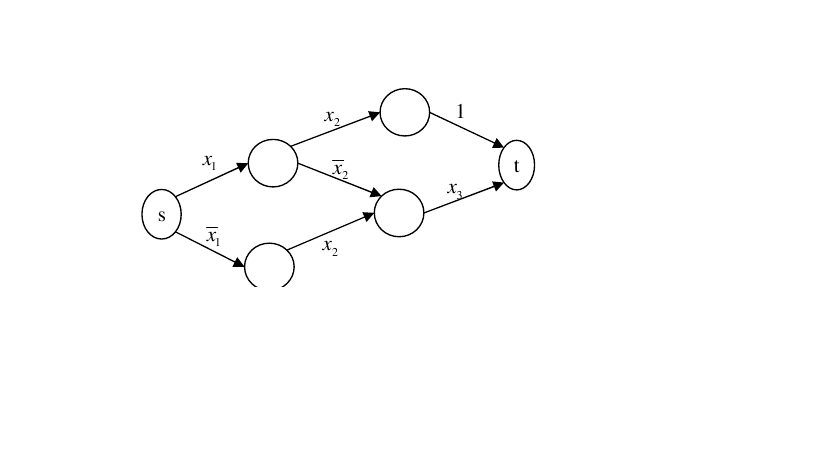
\includegraphics[scale=0.5]{majority} 
\caption{majority branching program}
\end{figure}.


\title{Barrington's theorem (3)}
Barrington's theorem shows, that any NC1-operation (include arithmetic ones), can be done with 5-width and poly-length branching program. For simulate such program on a quantom computer, we can label each "column" with the states $\ket{000}...\ket{100}$, and create simple unitary matrices for each branch, that extract the relevant qubit from the input, change the state of the 3 ancilla bits according to it. 

Start with 3 clean qubits at state 000, we expect to end in the same state at the end of this circuit process (and otherwise - we reject).


\title{The algorithm itself - closure}
\begin{itemize}
\item Concluding the above discussion, we can efficiently isolate the left-most bit using arithmetic operations.
\item however, we have to develop a method for saving all the other qubits as well. To isolate the $i$th qubit, we will first isolate the first qubit. if it was one, we will subtract $f_{n+1}$ from the input. Then, we can isolate the second-leftmost qubit by asking whether the remaining number is bigger then $f_{n}$ or not. If yes - the second qubit is *, and before isolate the third qubit we will subtract $f_{n}$, and so on... (The calculation of Fibonacci itself is of course in NC1, but it can be hard-coded into the circuit as well).
\end{itemize}






\section{The Hardness of computing Jones polynomial}
\subsection{The reduction from trace estimation to Jones polynomial evaluation - an overview}

We are now moving from showing an algorithm for estimate Jones polynomial of a trace closure of a braid at the point $\frac{2{\pi}i}{5}$, into showing that this is indeed a DQC1-hard problem. Specifically, we will want to show a reduction from trace-estimation to this estimation problem.

Say that we have some unitary matrix (with suitable quantom cicruit). How to reduce this problem to the Jones polynomials world?

We will have to construct some braid, of our choice, and show a correlation between of Jones polynomial and that circuit trace.

Since the only correlation we know so far between Jones Polynomial and quantom circuit is the Fibonacci representation, we will obviously have to approximate each quantom operation from the circuit C via Fibonnaci representation on some braid. For this, it is required to prove that Fibonacci representation matrices are dense, and we will prove that in subsection 3.2

More explicitly, we will show that $\{rho^{n}}_{**}$ is dense subgroup of $SU(f_{n-1})$, and that $\{rho^{n}}_{*p}$ is a dense subgroup of $SU(f_{n})$.

Next, we are tackeling the problem of the representation of qubit as braid with */p symbols. Since in our model there cannot be two adjacent $*$ symbols, a naive one-to-one mapping is not feasible.

Taking into account the fact that any such representation will have to give an "equal whight" to the different strings matching 0 and 1, and that we want to be able to operate on all the qubits freely, yields an optional encoding: $1 \rightarrow ppp, 0 \rightarrow p*p$.

However, there are many groups of three symbols, most of them aren't encode to anything, and we still want to know ahead what is the place that encode to each qubit abd qubit. We note that the probability that such group of three won't appear in $O(logn)$ bits is polynomially small. Therefore, we can assume that in every group of $O(\log{n})$ symbols we will find an encoding to one or to zero.

Notice that the Fibonacci matrix representation to $O(\log{n})$ bits is polynomial, so we will be able to actually construct these matrixes.

By the density theorem which will be proven in section 3.2, we now that there is some braid that suit to that matrix circuit. However, the number of crossing in the braid might be large. In section 3.3 we will prove that $poly(n)$ crossings in that braid is enough for any level of approximation that we want.

However, two issues are still remain.

First, we will show that Fibonacci matrices that act on string which start at $*$ are dense. But what we do in the case that there is no $*$ around?. Note that for the first 2 blocks, we can assume that there is a "*" in the middle of them (since it happens with a constant probability, we can make the other options to not contribute to the final trace, similar to what we did in section 1, with ancilla qubits and CNOTs). However, this method cannot be applied to all the blocks (since we will need polynomial number of ancila qubits, which we cannot have in DQC1 reduction).

Therefore, a method one can try is to "move the $*$". Specifically, we can imply a unitary transformation that "switches" between two segments in the center of two neigthboring blocks, if they are both in the same size, and both starts and end with a "p". (Since its just a replace action - its obvious that this matrix is indeed unitary). Note that:
\begin{itemize}
\item Since this matrix act on two blocks, its size is still polynomial.
\item Using this matrix we can bring a "*" to every block: At the start we have * in the middle of the first two blocks. Using this matrix once we can move the "*" to be in the first and the third blocks. Use it again, and we can move the "*" to be in the center of the second and the third blocks, and etc.
\item The probability that we wont find such "p" segment to make the replace on is polynomially small. Furthermore, the probability that our encoding lies within these segments is also polynomially small. Thus, we can assume that these conditions always hold, and add polynomially small error to the calculations. 
\end{itemize}

The second issue that we have to take into account, is the fact that the weight that the trace gives to each encoding is the same, while the weight that the Jones polynomial calculation gives is not. This issue can be solved by adding  one more superblock at the end. This superblock encoding will match the encoding of a matrix that, conditioned on the last original bit (i.e. just if it was "p"), rotate the state, so the inner product of the new state with the old state is exactly $\frac{1}{\phi}$ (recall that in the Jones polynimial calculations, the weight we gave to the "ending with p states" was $\phi$). The orthogonal part of the state after the rotation will obviously wont contribute to the trace, and therefore we will get in the Jones polynomial calculation that its value is equal to the trace in the original circuit.

This completes the proof that the Jones polynomial estimation is hard in DQC1 (except proving the theoremes in sections 3.2 and 3.3). 
\subsection{Fibonacci representation gates are dense}
In this section we will prove that the Fibonacci representation gates are dense. Specifically, we will prove that:
\begin{itemize}
\item ${\rho^{n}}_{**}$ (which stand for all the Fibonacci matrices, taken over the subspace of strings with start and end with *), are dense in $SU(f_{n-1})$
\item ${\rho^{n}}_{*p}$ (which stand for all the Fibonacci matrices, taken over the subspace of strings with start and end with *), are dense in $SU(f_{n})$
\end{itemize}

Together, this two statements implies the fact that as long that our encoding start with "*", we can find a suitable Fibonacci matrix that will approximate any unitary transformation on our n bits.

First, lets remind what the term "dense" means. 
\title{density- definition}
A subset of gates $\in SU(f_{n+1})$ is said to be dense, if we can approximate any gate in $ SU(f_{n+1})$ by this subset. Formally, we can measure the distance between 2 unitary matrices by their trace distance: 
$D(\sigma, \rho) = \frac{1}{2}Tr[\sqrt{(\rho - \sigma)^{\dagger}(\rho - \sigma)}]$
, and define a set of gates to be $\epsilon$-dense if for every unitary matrix there is a gate from the group (or can be built by the group) which is $\epsilon$ close to it.

We will prove that therorem by induction on n. The base case is to prove that ${\rho^{4}}_{**}$, ${\rho^{3}}_{*p}$ are dense in $SU(2)$. How to prove density in $SU(2)$?

For that we will use an isomorphism from $SU(2)$ to $SO(3)$ - the group of rotations on the sphere with radius 1.


\subsubsection{SO(3) and the connection to density}

\title {The SO(3) group and its subgroups}
The SO(3) group is defined to be the rotation group in the unity circle. That is, each element in SO(3) is defined by its rotation degree $\tetha$ and by its axis or rotation (x,y,z). Note that we can easily find isomorphism $\phi$ from the single qubit operations SU(2) to the rotation group: we can write each 2x2 unitary matrix as $cos(\frac{\tetha}{2}I + \frac{\thetha}{2}{a\sigma_{x} + b\sigma_{y} + c\sigma_{z}})$, which correlates each unitary operation to a degree $\thetha$ and an axis of (a,b,c). For a general group of gates G, it is obvious that if ${\phi(x) for x \in G}$ does not contained in any finite subgroup of SO(3), then it will actually be able to create ALL SO(3), which means that after the isomorphism the results will be "dense in SO(3)", which will make the original kernel dense in SU(2).

Therefore, we have to determine what the finite subgroups of $SO(3)$ looks like.

\begin{itemize}
\item Consider such subgroup $G \subset SO(3)$. Each element $g \in G$ is an action that rotates some point on a sphere, to some other point on that sphere. 
\item Since its a rotation, each action should have 2 "poles" - points which stay invariant after the rotation is taking place.
\item We will say that two poles $p, p^{'}$ are equivalent, if there exist some action $g \in G$ such that $g \circ p = p^{'}$, and noate this classes by $C_{1}...C_{M}$.
\item Note that if $p, p^{'}$ are equivalent with some action $g$, then any action $h$ which leaves $p$ in place, can be used to obtained an action $g \circ h$ which send $p$ to $p^{'}$.
\item In addition, note that neceessarily $p$ and $p^{'}$ stay invarant under the same number of operations, since ($g, h$ defined as before) $ghg^{-1}$ is an action which $p^{'}$ is its pole: $ghg^{-1}p^{'} = ghp =gp = p^{'}$.
\item from all the above, we get the relation: $|C_{i}| = \frac{N}{n_{i}}$, when $n_{i}$ is the number of operations that leaves some pole $p$ in place, and N is the number of elements in G.

\item In addation, note that $\sum\limits_{1..M}{C_{i}(n_{i} -1)} = 2(N-1)$, since the left side contains the number of poles, when each pole is multiplied by the non-trivial elements that leaves it fixed, and any element from the $N-1$ non trivial elements has 2 poles.

\item the combination of the two formulas from abobe yields the following restriction on the SO(3) subgroups: $\sum\limits_{1..M}{1 - \frac{1}{n_{i}}} = 2(1-\frac{1}{N})$.

\item This solution has only 5 options:
\item $M=2, n_{1}=n_{2}=N$. this solution describes a subgroup of size N, contains cyclic rotation of $\frac{2{\pi}i}{N}$ around the same circle.
\item $M=3, n_{1}=n_{2}=2, n_{3}=\frac{N}{2}$. This solution describes a dehideral group (imagine a regular cyclic group with size N, that we add to it all the reflections of each element as well).
\item $M=3, n_{1}=2, n_{2}=n_{3}=3, N=12$, describes a tetrahedron.
\item $M=3, n_{1}=2,n_{2}=3, n_{3}=4, N=12$, descrobes octahedron,
\item $M=3, n_{1}=2, n_{2}=3, n_{3}=5, N=60$, decribes dedocahedron.
\end{itemize}

Notice that in the last 3 finite subgroups, the largest order possible for some element is 5. We will use this fact later. 

Now, after we know that, lets return to the density therorem proof.

As for the ${\rho^{4}}_{**}$ case, its defined 2 matrices:

${\rho^{4}}_{**}(\sigma_{1}) = {\rho^{4}}_{**}(\sigma_{3}) = \begin{pmatrix} b & 0 \\ 0 & a \end{pmatrix}$

${\rho^{4}}_{**}(\sigma_{2}) =  \begin{pmatrix} c & d \\ d & e \end{pmatrix}$

Since global phase does not interent us, we can normalize these matrices to have determinant of one, thus being a subgroup of $SU(2)$. we get the matrices:

$A = \frac{1}{\sqrt{ab}} \begin{pmatrix}  b & 0 \\ 0 & a \end{pmatrix}$
and:
$B = \frac{1}{\sqrt{ce - d^{2}}}  \begin{pmatrix} c & d \\ d & e \end{pmatrix}$

after imply the isomorphism $\phi$ on these matrices, we get a rotation by angle of $\frac{7{\phi}}{5}$, by different axes. The angle between these axes is $\tetha_{12} = cos^{-1}(2 - \sqrt{5}) = 1.809$.

All that remain is to show that this subgroup of $SU(3)$ is not contained in any final subgroup. First, note that this subgroup has two diferent rotation axes, therefore it cant be contained in one of the first two options, for every N. Second, note that ${\phi(A)}^{5}{\phi(B)}^{5}$ is a rotation by $2\thetha_{12}$. (This is because ofter 5 rotations of $\phi(A)$ we get rotation by $7\phi$ arount the first axe (which is equal to the "mirror" around to this axe, and after 5 rotations more of $\phi(B)$ we will get a mirror around the second axe - similar to whats going on in the groover algorithm). Direct checking shows that this rotation order in $SO(3)$ is more then 3, therefore  it cant be contained in any of the last 3 finite groups. This completes the proof that  ${\rho^{4}}_{**}$ is dense in $SU(2)$ (up to a phase). 

As a result, the fact that ${\rho^{3}}_{*p}$ is dense in  $SU(2)$ immediatly follows (the two matrices of ${\rho^{3}}_{*p}$  are identical to the two matrices of ${\rho^{4}}_{**}$ ).

We are now moving to prove the induction step. First, we take a closer look at  ${\rho^{n}}_{**}$. We note that we can split each matrix in ${\rho^{n}}_{**}$ to two matrices - one that act on the subspace ending with *p* like the original matrix, and one that act on the subspace pp* like the original matrix. By definition $\rho^{n}_{**}(\sigma_{1}) ... \rho^{n}_{**}(\sigma_{n-3})$ will not "mix" these subspaces.

Furthermore, since each $\sigma_{i}$ like this affects only the neigboring "bits", it holds that there is one to one correspondense between $\rho^{n-2}_{**}(\sigma_{1}) ... \rho^{n-2}_{**}(\sigma_{n-3})$ and $\rho^{n}_{*...*p*}(\sigma_{1}) ... \rho^{n-2}_{*...*p*}(\sigma_{n-3})$, 

and one to one correspondence between $\rho^{n-1}_{**}(\sigma_{1}) ... \rho^{n-1}_{**}(\sigma_{n-3})$ and $\rho^{n}_{*...pp*}(\sigma_{1}) ... \rho^{n}_{*...pp*}(\sigma_{n-3})$ .

However, $\rho^{n}_{**}(\sigma_{n-2})$ will mix these two subspaces, since it will affect the $n-1$ symbol.

We will inroduce two lemmas that will help us proving, that the above analysis actually implies that ${\rho^{n}}_{**}$ is dense.

The first lemma that we need is the bridge lemma: we saw that the subspace ** can be devided to two subspaces, when we know that  ${\rho^{n-1}}_{**}$ and ${\rho^{n-2}}_{**}$ are dense in them. We also saw that $\rho^{n}_{**}(\sigma_{n-2})$ mixes these subspaces. We will want to show that it means something about $\rho^{n}_{**}$ density in $SU(f_{n-1})$. 

\subsubsection{The bridge lemma}
Consider a linear space C which is a direct sum of two orthogonal subspaces A and B, and assume that dimB > dimA ≥ 1.
Let W be a bridge transformation between A and B. Then any U ∈ SU(C) can be
approximated to an arbitrary precision using a finite sequence of transformations from
SU(A), SU(B) and W. Consequently, the group generated by SU(A), SU(B) and W
is dense in SU(C).

Here A and B are of course $SU(f_{n-3}), SU(f_{n-2})$, C is $SU(f_{n-1})$, and the bridge element is  $\rho^{n}_{**}(\sigma_{n-2})$.

However this is not enough! We indeed know that the space  $SU(f_{n-1})$ can be devided to two parts, such that  $\rho^{n-2}_{**},  \rho^{n-2}_{**}$ are dense in them.... but after we "combine" these operations together, we might get some dependecy: i.e, we will be able to get every matrix from $SU(f_{n-3})$, but the matices we will use will prevent us from get some of the matrices in $SU(f_{n-2})$ (and vice versa...).

To resolve that issue, we will have to inroduce the decoupeling lemma:

However, this is still not enough: indeed, we now that 
\subsubsection{The decoupling lemma}
Let G be an infinite discrete group, and let A, B be two finite Linear spaces with different dimensionality. Let $\tau_{a}$ and $\tau_{b}$ be
two homomorphisms of G into SU(A) and SU(B) respectively and assume that $\tau_{a}(G)$
is dense in SU(A) and $\tau_{b}(G)$ is dense in SU(B). Then for any U ∈ SU(A) there exist
a series {σn} in G such that
$\tau_{b}(σn) → U$
$\tau_{b}(σn) → 1$


Using this final lemma we will be able to finally complete the proof of the density of  $\rho^{n}_{**}$:

Base case: clearly $\rho^{3}_{**}$ is dense in $SU(1)$ (which include only one matrix).
            We showed that $\rho^{4}_{**}$ is dense in $SU(2)
            
Step: Assume that  $\rho^{n-2}_{**}(B_{n-1})$ is dense in $SU(f_{n-3})$, and  $\rho^{n-2}_{**}(B_{n-1})$ is dense in $SU(f_{n-2})$, and we would like to prove that  $\rho^{n}_{**}(B_{n})$ is dense in $SU(f_{n-1})$. By the fact observed above $\rho^{n-2}_{**}(\sigma_{1}) ... \rho^{n-2}_{**}(\sigma_{n-3})$ remains unchanged when moving to  $\rho^{n}_{**}$. Therefore, by the induction assumption and the decoupeling lemma, using $\rho^{n}_{**}$ we can approximate any $U \oplus 1$ when $U \in SU(f_{n-3})$, and any  $1 \oplus U$ when $U \in SU(f_{n-2})$,

By the bridge lemma, this fact (and the fact that we use  $\rho^{n}_{**}(\sigma_{n-2})$ as a "bridge"), is enough for claiming that  $\rho^{n}_{**}(B_{n})$ is dense in $SU(f_{n-1})$.

\end{document}

